\documentclass[thesis.tex]{subfiles}

\chapter{Giới thiệu về nhận dạng người nói}

Trong chương này, tác giả giới thiệu tổng quan về bài toán nhận dạng người nói, điểm qua các nghiên cứu liên quan và giới thiệu về bài toán trong đồ án.

\section{Giới thiệu chung về bài toán nhận dạng người nói}

Nhận dạng người nói (speaker recognition) là quá trình tự động nhận dạng người đang nói bằng cách sử dụng thông tin riêng biệt của người nói đó có trong tín hiệu âm thanh. Nhận dạng người nói được ứng dụng rộng rãi trong nhiều lĩnh vực khác nhau, tuy nhiên cũng gặp không ít khó khăn khi triển khai trong thực tế. Do vây, nghiên cứu bài toán nhận dạng người nói rất được quan tâm bởi nhiều nhà khoa học trên thế giới. Một số ứng dụng của bài toán có thể kể đến như:

\begin{itemize}
    \item Bảo mật cho các hệ thống tài chính, ngân hàng: người dùng dùng giọng nói kết hợp với các lớp bảo mật khác cho xác thực để tăng tính bảo mật khi giao dịch.
    \item Tăng trải nghiệm khách hàng trong tổng đài chăm sóc khách hàng.
    \item Xác định danh tính tội phạm trong an ninh khi thu được dữ liệu giọng nói.
    \item Kết hợp với các hệ thống nhận dạng tiếng nói để xây dựng ứng dụng gỡ băng cuộc họp.
    \item ...
\end{itemize}

Dựa vào ứng dụng, nhận dạng người được phân loại thành nhận định người nói (speaker identitfication) và xác minh người nói (speaker verfication) (Hình \ref{fig:verification-identification}). Trong nhận định người nói, một đoạn tiếng nói từ một người không xác định được phân tích và so sánh với mô hình giọng nói của những người đã biết. Người này được nhận định là người mô hình giọng nói phù hợp nhất với câu nói đầu vào. Trong xác minh người nói, một người lạ xác nhận một danh tính đã biết; đoạn tiếng nói của người này được so sánh với mô hình giọng nói của danh tính đang được xác nhận. Nếu điểm tương đồng đủ tốt, nghĩa là trên một ngưỡng nào đó, danh tính của người lạ được chấp nhận. Ngưỡng cao khiến những kẻ mạo danh khó được chấp nhận bởi hệ thống, nhưng có nguy từ chối nhầm người dùng hợp lệ. Ngược lại, ngưỡng thấp cho phép chấp nhận người dùng hợp lệ một cách nhất quán, nhưng có nguy cơ chấp nhận những người giả mạo. 

\begin{figure}[h]
    \centering
    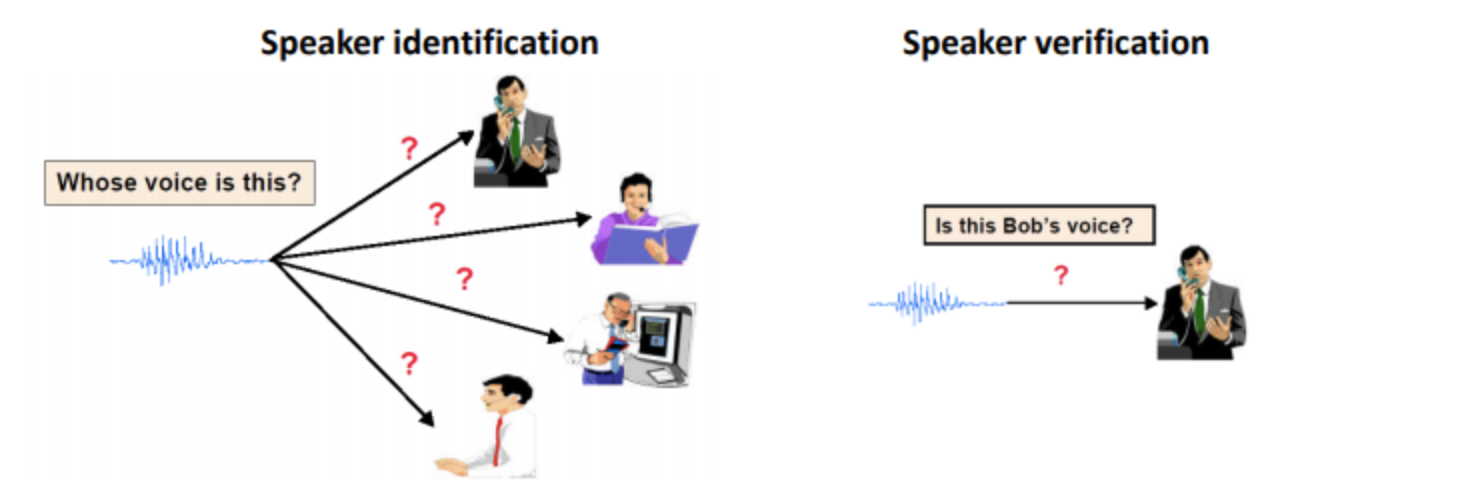
\includegraphics[width=0.9\textwidth]{images/identification-verification.png}
    \caption{Nhận định người nói và xác minh người nói}
    \label{fig:verification-identification}
\end{figure}

Thông thường, hệ thống nhận dạng người nói được chia thành 3 pha như mô tả trong Hình \ref*{fig:overall-system}

\begin{itemize}
    \item Pha 1: phát triển (development). Trong pha này, mô hình có khả năng biểu diễn đặc trưng người nói được huấn luyện và tối ưu trên một cơ sở dữ liệu các đoạn tiếng nói.
    \item Pha 2: ghi danh (enrollment). Trong pha ghi danh, biểu diễn của người dùng mới được trích xuất bằng mô hình phát triển ở pha 1 và lưu trữ trong cơ sở dữ liệu để phục vụ cho pha 3.
    \item Pha 3: kiểm tra (testing). Với bài toán nhận định người nói, vec-tơ biểu diễn của câu nói đầu vào được so sánh với tất cả biểu diễn trong cơ sở dữ liệu để tìm ra người dùng tương đồng nhất. Trong bài toán xác thực người nói, được cung cấp danh tính đầu vào, hệ thống chỉ so sánh đoạn tiếng nói đầu vào và đoạn của danh tính trong hệ thống để đưa ra quyết định.
\end{itemize}

\begin{figure}[h]
    \centering
    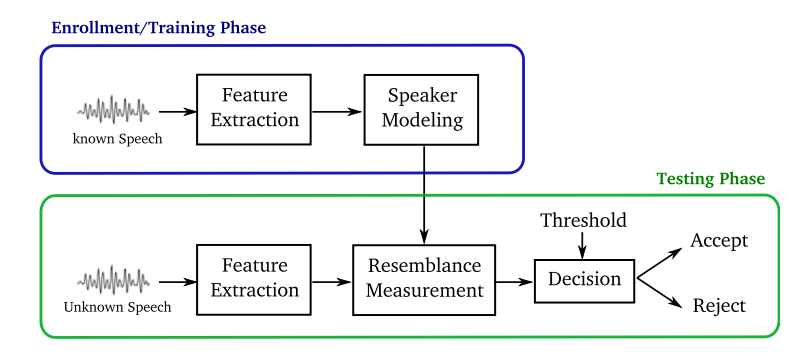
\includegraphics[width=0.9\textwidth]{images/overall-system.png}
    \caption{Tổng quan hệ thống nhận diện người nói}
    \label{fig:overall-system}
\end{figure}
\TODO{Vẽ lại hình này và include development phase to make it more clear}

Trong thực tế, hiệu năng của hệ thống nhận diện người nói bị suy giảm do sự khác biệt của các kênh và phiên giữa tín hiệu giọng nói trong pha ghi danh và pha kiểm tra. Các yếu tố làm ảnh hưởng tới tín hiệu giọng nói bao gồm:

\begin{itemize}
    \item Sử dụng các loại micrô khác nhau khi thu tín hiệu đăng ký và kiểm tra.
    \item Điều kiện tiếng ồn và độ vang của môi trường.
    \item Sự khác biệt trong giọng nói của người nói ở các giai đoạn khác nhau của độ tuổi, sức khoẻ, phong cách nói và trạng thái cảm xúc.
    \item Các kênh truyền như các loại điện thoại di động khác nhau, micrô, giao thức truyền âm thanh qua internet có thể làm thay đổi giọng nói.
\end{itemize}

Dựa vào sự tương đồng của các câu nói đầu vào, phương pháp giải quyết bài toán nhận dạng người nói còn có thể chia thành nhóm dựa vào văn bản (text-dependent speaker recognition - TDSR) và nhóm không dựa vào văn bản(text-independent speaker recognition - TISR). Các hệ thống TDSR yêu cầu người nói cung cấp các đoạn tiếng nói có nội dung theo một từ hoặc câu được định sẵn; nội dung các câu nói phải được giữ nhất quán trong cả quá trình huấn luyện và nhận dạng. Ngược lại, TISR không yêu cầu người dùng phải thu theo bất cứ một văn bản nào. Với các đoạn tiếng nói ngắn, các hệ thống TDSR đã có thể đạt được hiệu suất nhận diện cao, trong khi các TISR yêu cầu các câu nói dài để huấn luyện các mô hình đáng tin cậy và đạt được hiệu suất tốt. Do sự bất tiện của các hệ thống TDSR, trong vài năm gần đây, cộng đồng nghiên cứu tập trung phát triển các mô hình học sâu end-to-end nhằm mục đích biểu diễn các đoạn tiếng nói ngắn.

\section{Nhận dạng người nói trong tiếng Việt}

\section{Mục tiêu và phạm vi đồ án}

\section{Bố cục đồ án}